\documentclass{article}

\usepackage{cite}
\usepackage{graphicx}
\usepackage{hyperref}

\title{Response to Reviewer Comments}
\date{2023 June}
\author{Mohammad Robati Shirzad and Patrick Lam}
\begin{document}


\maketitle

Please find below our response to the reviews for our EMSE submission ``A Study of Common Bug Fix Patterns in Rust''.

\section{Introduction}

We thank the reviewers for the thoughtful reviews. We first provide summaries here, followed by detailed responses below.

\subsection{Methodology \& Experiments}

In response to reviewer questions about methodology and experiments, we further explain our methodology and discuss why we made the choices we did. We summarize here, but invite the reviewers to read our full responses in Section~\ref{sec:detailed} of this response. We hope that the reviewers can better understand why we believe our choices to be appropriate. (Hyperlinked references in this document refer to parts of the response, while un-linked references are to the paper).\\ 

Reviewer 1:
\begin{itemize}
    \item Order information: our dataset is not large enough to incorporate it (\ref{rev:1:order}).
    \item Ignoring terminal tokens: including information about terminals would have led to dimensionality in the millions, which would be infeasible in terms of computational complexity (\ref{rev:1:terminal}). 
    \item RQ1: we have included qualitative comparisons of our approach with previous approaches and discussed how our approach is superior to those approaches. (\ref{rev:1:rq1}).
\end{itemize} 

Reviewer 2:
\begin{itemize}
    \item Context: we believe our results show that context is not required to get meaningful results (\ref{rev:2:embedding}).
    \item Leaf nodes and penalizing large diffs: any clustering approach is going to have trouble clustering together large diffs, which have more ways to differ from each other than small diffs (\ref{rev:2:embedding}). 
    \item Picking 50 datapoints: manually evaluating large clusters is infeasible---e.g. we do not have the resources to evaluate the cluster with 618 datapoints manually (\ref{rev:2:minor}).
\end{itemize}

In summary, we believe that we have made the best possible design decisions given limitations in datasets and resources available to us, and that our results are strong enough that they support our decisions.

\subsection{Discussion}

We wholeheartedly agree that it is important to show that the identified patterns are valuable. We have added Section 4.1, “Patterns Present and Missing” (specifically discussing the value of the top 10 patterns and summarizing our learnings) and Section 4.2 “Usefulness of Rust Bug Patterns” (discussing the general usefulness of patterns), as well as paragraphs on actionability to 6 of the groups of patterns. 

\subsection{Clarity}

Thanks for the suggestions! We have added many of the suggested changes to the text of the paper. We have explained some of the reviewer questions in this response. If a reviewer thinks that those responses should be in the paper itself, or requires further clarification, we are happy to oblige.

\section{Detailed Responses}
\label{sec:detailed}
We have reproduced all of the reviewer comments below (in italics) and discuss them in detail. Once again, thanks for the detailed reviews.

\subsection{Reviewer 1}

\textit{This paper conducts a study on bug-fix patterns of the language Rust. Rust is a system-level programming language that has attracted huge attention among developers. Rust is specially designed to help developers to avoid illegal memory operations which are easily introduced in C/C++ programs. It has several particular language features, so the bugs in Rust may also have subtle differences from other programming languages. Thus it is important to study the bug's unique features and trends in Rust.
To perform the study, the authors collect bugs and their corresponding patches from GitHub. Then they embed the patches to vectors that have the same length, and cluster the vectors. At last, they manually analyze the groups and extract fix patterns.
This paper is very well-written and organized. The scale of this study is sufficient and the workflow is overall reasonable. In addition, this paper firstly studies Rust fix patterns, and it proposes a novel embedding method for Rust program diffs (i.e., patches). To this end, I think the significance of this paper is guaranteed.However, I would like to mark this paper as a major revision, with the following concerns.}

\subsubsection{\label{rev:1:order}The order information}

\noindent \textit{\textbf{R1:} The embedding lacks order information, which could be simply appended a vector with a sequence representing the occurrence list of the AST nodes.}

\vspace*{1em} \noindent \textbf{Response:} Yes, our embedding lacks order information in the dimensions. We do not believe that order information would be useful here. Our application is bug categorization, and previous works on bug categorization obtained reasonable results without ordering. If we wanted to include ordering in the embedding, we would need a neural model, but our dataset is not large enough to train a neural model that can fully understand the structures of Rust programs. 

To elaborate: simply appending a vector representing the occurrence list of AST nodes wouldn't be compatible with DBSCAN, which requires fixed-sized inputs for clustering. AST paths are inherently variable-sized.

code2vec~\cite{alon2019code2vec} does manage to create an order-sensitive embedding. However, code2vec uses neural networks to generate embeddings by training them on a 30GB dataset. Its goal is to predict certain code elements, such as method names. That is not our goal.

To apply a code2vec-style approach, we would need to create a dictionary of all possible paths within an AST, and then provide the neural network with observed paths from our target programming language.

We instead chose to follow previous bug categorization work (for JavaScript~\cite{hanam2016discovering} and Python~\cite{yang2022mining}), and simply use a feature vector to represent code differences, rather than neural-based embeddings. Earlier researchers chose feature vectors for similar reasons as we did: the nature of the bug categorization task, and dataset limitations. \\ \\

\subsubsection{\label{rev:1:terminal}Ignoring the terminal tokens}

\textit{\textbf{R1:} In addition, ignoring the terminal tokens has advantages and disadvantages, and it is better to evaluate by experiments. }

\vspace*{1em} \noindent \textbf{Response:} We appreciate the value of empirically validating design decisions when possible. However, in our case, not ignoring terminal tokens (variable names and constant values) would have been impractical, due to the high dimensionality (millions) of the resulting embedding vectors. The cost of processing such data would be prohibitive in both time and space. We judged that the likelihood of improvements was unlikely to justify the significant engineering effort required to get DBSCAN (which is $O(n~\mbox{log}~n)$) to work with that magnitude of sparse data.

code2vec-style neural embedding could mitigate the high dimensionality; we could create a separate dictionary specifically for variable names (terminals) and generate embeddings by concatenating values from both the variable names dictionary and the paths dictionary. This way, the resulting embedding would incorporate knowledge from both nonterminal and terminal elements of the AST. However, as discussed above, we chose a feature vector rather than a neural embedding, following previous work, because a neural embedding would be overkill for bug categorization and because of dataset limitations. \\ \\

\subsubsection{\label{rev:1:patch}Illustrating patch to vector transformation}

\textit{\textbf{R1:} It is better to add an example to illustrate the procedure of transforming a patch to a vector, i.e., use an example patch in Section 2 to link all the processing procedures.}

\vspace*{1em} \noindent \textbf{Response:} Thanks. We have made the example in Section 2 much more explicit and added some previously-missing steps to Figure 2 (namely the essence of change vector) as well as text linking Figures 1 and 2. Section 2 now contains a complete running example of transforming a patch to a vector. This example is in Sections 2.1.2 and 2.1.3. We describe the example in paragraphs labelled “Running example” throughout these subsections. We are happy to pull the motivating example into its own subsection if the reviewer thinks that is most appropriate. \\ \\

\subsubsection{\label{rev:1:conclusion}Conclusion of the patterns}

\textit{\textbf{R1:} The highlighted conclusion of the pattern is missing. I expect to know which part is more likely to be buggy and want to know several typical examples.}

\vspace*{1em} \noindent \textbf{Response:} The new Section 4.1 (``Patterns Present and Missing'') summarizes the patterns that we found and their overall usefulness. We also added an “actionability” section to eight of the patterns to discuss them in further detail and how they can aid a repair tool. \\ \\

\subsubsection{\label{rev:1:compare}Comparing the discovered patterns to other languages}

\textit{\textbf{R1:} Also, I expect to see the bug patterns that are unique in Rust programs, and further discussions about the differences with other languages like C, C++, Python and Java. }

\vspace*{1em} \noindent \textbf{Response:} The BC-related patterns are unique to Rust programs because they concern Rust's unique borrow checker. On the other hand, 11 of the 12 general patterns (excluding G.option) have counterparts in other widely-used programming languages, and we discuss differences in the text.

Specifically, we have added content to Section 3.2.1 about similarities and differences between the Rust attribute bug pattern and Python decorators/Java annotations. Section 3.2.5 relates Rust traits to Java interfaces and shows an example of how traits are more complicated. Section 3.2.6 explains how Rust's match generalizes C-style switch statements. \\ \\

\subsubsection{\label{rev:1:rq1}Concerns about RQ1}

\textit{\textbf{R1:} The answer to RQ1 is not persuasive. Although the most important AST node can be somehow regarded as the most representative part of a patch, the relationship is not that strong to get the answer. It is better to compare with existing approaches and design a better metric to measure the performance.}

\vspace*{1em} \noindent \textbf{Response:} We understand your concern regarding the persuasiveness of the answer to RQ1. We've acknowledged this limitation in our study and our threats to validity section mentions it up front (``our code embedding approach\ldots''). While it is true that the relationship between the most important AST node and the most representative part of a patch may not be exceptionally strong, we designed our approach to prioritize the non-terminals that are important, and we sought to examine the connection between those important non-terminals and actual code changes.

We'd like to point out that previous work, such as the bug pattern studies for JavaScript~\cite{hanam2016discovering} and Python~\cite{yang2022mining}, each only introduced one embedding method to compute code change vectors that produced meaningful clusters, and there was no comparison between different embedding methods in those works.

In contrast to the existing embedding approach proposed by Hanam et al.~\cite{hanam2016discovering}, where they introduced the Feature Properties table leading to an order-sensitive embedding but sparse datapoints, our approach results in 11x denser datapoints (Section 5.4), which implies smaller storage requirements and better DBSCAN performance. The feature vector proposed for Yang et al.~\cite{yang2022mining} focuses only on single-hunk bugs and includes information such as the number of variables, lines, and function arguments. Our approach is more general: it handles multiple-hunk commits.

In our RQ1 experiment, we opted for a manual inspection process where the two authors, who possess Rust knowledge, reviewed the vector and its corresponding code change to verify representativeness. While this manual approach may not be as statistically rigorous as an automated inspection (because it inspects smaller numbers of points), we considered it to be an intuitive and straightforward method.

Of course, an automated inspection could examine more code examples. Such an inspection would also be subject to the validity threat of embedding assumptions about what to inspect. And, developing an automated code comprehension tool specifically for Rust, capable of interpreting code changes and providing explanations for the reasons behind those changes, poses a significant challenge. Such a task would itself require a separate and comprehensive study. We believe that developing an automated inspection tool would be a distraction and would not contribute to answering the core questions about Rust bug patterns behind this work.

We further emphasize that our code embedding approach is only the initial step in our bug categorization pipeline. We had to choose a specific embedding method to create our code diff vectors: different embedding approaches would lead to entirely different datasets and possibly different clustering outcomes. Each embedding approach would require separate manual analysis of the resulting clusters. Consequently, we made the decision to select one embedding method and to validate it.

To additionally justify our choice of embedding approach, we evaluated whether the clusters generated by our approach contained dissimilar data points, as this was a critical factor in determining its suitability. Our bug categories demonstrate that our clusters successfully encompass cross-project bugs, and this can be verified by examining the introduced code changes in our replication package. \\ \\

\subsubsection{\label{rev:1:bib}Adding more bibliography}

\textit{\textbf{R1:} Several patch/code/text embedding works should be discussed in the section of related work.}
\begin{enumerate}
    \item Automated Classification of Overfitting Patches with Statically Extracted Code Features. (TSE 2019)
    \item Is this Change the Answer to that Problem? Correlating Descriptions of Bug and Code Changes for Evaluating Patch Correctness. (ASE 2019)
    \item Context-Aware Code Change Embedding for Better Patch Correctness Assessment. (TOSEM 2022)
    \item CC2Vec: Distributed Representations of Code Changes. (ICSE 2020)
    \item code2seq: Generating Sequences from Structured Representations of Code. (ICLR 2019)
    \item BERT: Pre-training of Deep Bidirectional Transformers for Language Understanding.
\end{enumerate}


\vspace*{1em} \noindent \textbf{Response:} Thanks. We have added 5 of these works to our related work section.

\subsection{Reviewer 2}

\textit{In this paper, the authors aim to mine and study bug-fix patterns in Rust programs. They discuss a new encoding method for Rust patches, which changes a patch into a vector. Then they apply a clustering algorithm to identify common patch patterns. In the end, they discuss 20 identified patterns.
Rust is a new, popular programming language, and studying its bug-fix patterns is important. However, I have some concerns about the methodology and the value of the identified patterns. I discuss my concerns as follows.} \\ \\

\subsubsection{\label{rev:2:value}The value of the identified patterns}

\textit{\textbf{R2:} The value of the identified patterns is unclear to me. The authors claim that they want to study bug-fix patterns in the title and in the methodology section. However, it is difficult for me to correlate the discussed patterns with any particular bug types. I cannot figure out any actions (e.g., how to build bug detection tools, how to inspect my Rust code) to take after reading the paper.}

\vspace*{1em} \noindent \textbf{Response:} The new Section 4.1 (“Patterns Present and Missing”) summarizes the patterns that we found and what one could do with them. We also added an “actionability” section to some of the patterns to discuss them in further detail and how they can aid a repair tool. We found that many of the patterns are interesting but still require further work to distill into a repair tool. \\ \\

\subsubsection{\label{rev:2:refactoring}Refactoring, not bug fixing}

\textit{\textbf{R2:} Moreover, many studied patterns are actually for refactoring purposes and compiler errors (not for fixing bugs).}

\vspace*{1em} \noindent \textbf{Response:} In Section 2.3.2 we discuss three types of changes: bug-fix, fix-induced, and refactoring, following the definitions of Cotroneo et al (2019). Our intention is to only consider bug-fixing and fix-induced commits, and we aimed to omit changes that were purely refactoring. However, some of the changes that we included may appear to be refactoring changes but actually have performance implications. We chose to specifically include those. For instance, \verb+BC.clone.ref+ does not alter the program's behaviour (no additional test cases pass) but can reduce CPU usage. Other changes, like adding Option to a type, can be considered refactorings, but are in support of bug fixes, and hence are fix-induced. \\ \\

\subsubsection{\label{rev:2:compile}Committing code with compiler errors}

\textit{\textbf{R2:} It is very rare for a programmer to submit a commit that makes a Rust program uncompiled.}

\vspace*{1em} \noindent \textbf{Response:} We agree, and Section 4.1 in our discussion acknowledges this point. \\ \\

\vspace*{1em} \noindent \textit{\textbf{R2:} Why does the first pattern in Section 3.3.3 show up in the study? The code before the patch in the first figure of Section 3.3.3 cannot be compiled.}

\vspace*{1em} \noindent \textbf{Response:} Whether the code compiles or not depends on the method signature of \verb+emit()+.

If \verb+emit()+ is like this:
    \verb+fn emit(&self, db: &DiagnosticBuilder);+
Then \verb+mut+  is not necessary.

If \verb+emit()+ is like this:
    \verb+fn emit(&mut self, db: &DiagnosticBuilder);+
Then the presence of \verb+mut+ is mandatory in the closure. 

In the example mentioned here, the presence of \verb+mut+ in the closure parameter \verb+|mut e|+ becomes necessary following a modification of \verb+emit()+ to require a mutable reference (\verb+&mut self+). The patch that we are classifying simultaneously changes \verb+emit()+ and the reference to add \verb+mut+ in both places. \\ \\

\subsubsection{\label{rev:2:embedding}Our embedding method}

\textit{\textbf{R2:} The method for encoding patches seems problematic to me. Giving leaf elements more weights prioritizes small patches. In section 3, all discussed patches are small patches without any information about what is the bug or the program context. My understanding is that almost all code in Section 3 before the patch is good code. They become buggy because they are used in particular contexts. Combining the patches together with the program contexts is more valuable.}

\vspace*{1em} \noindent \textbf{Response:} Let's first talk about the issue of context. We agree that a bug is only a bug in a particular context. We understand that the reviewer is saying: had we considered the statements around a bug fix, then we would have gotten better results than just considering the bug fix itself in isolation. 

We point out that Ruxanne considers changes that developers have labelled as bug-fixing changes (or fix-induced changes). Part of our thesis is that, given a change labelled as a bug-fixing change, the AST diff is enough to permit classification of that bug, and that context is not required. We believe that our results show that it is indeed enough: we identified 12 general patterns and 8 borrow-checker patterns based on the information we collected.  Section 3 provides links to the changes, so that the reader can examine the changes themselves. 

We'd ask the reviewer to consider our results on their own merits, rather than thinking about a possible other approach that also could have worked. It is possible that more information, as the reviewer suggests, gives better results, but it also may overfit, for instance, and computations are harder with more data. In our response to Reviewer 1, we discussed the embedding approaches taken by the Python~\cite{yang2022mining} and JavaScript~\cite{hanam2016discovering} related works.

Having said that, Ruxanne does consider the parents in the AST when reasoning about a change. It does not specifically consider siblings of a change in the AST, which is the context that we believe the reviewer is talking about. For instance, in Figure 1, the \verb+head.clone()+ change paths include the addition of the method call node to the path containing the nonterminal \verb+head+, as well as the addition of the path containing the \verb+clone()+ call. We consider both of those paths from root to leaf, shown as Paths 2 and 3 in the Figure.

As for the comment about small patches and leaf nodes, we'd like to clarify the role of the weights. We performed a preliminary step to determine fixed weights for different types of AST nodes. We then used these weights, uniformly across our data set, to compute essence-of-change vectors (as depicted in Figure 2). Both small and large patches have their occurrences vectors multiplied by the same weights, giving essence-of-change vectors. RQ1 validates this essence-of-change computation. In subsequent steps, we then cluster the essence-of-change vectors to find bug patterns. 

We acknowledge that it is possible that a large patch may be harder to cluster, because it has to look like other patches.  Additionally, we believe that any clustering-based approach is likely going to have large diffs be further apart for the same reason that ours does: there's just more going on. But there is nothing inherently penalizing a larger diff. Also, we point out that the related work by Pan et al specifically excludes diffs with seven statements or more, while we allow them. \\ \\

\subsubsection{\label{rev:2:ast}AST Transformation}

\vspace*{1em} \noindent \textit{The implementation described in Section 2.1 is difficult to follow.}

\vspace*{1em} \noindent \textit{\textbf{R2:} First, I don't understand how an AST is transformed to a dictionary in Section 2.1.1.}

\vspace*{1em} \noindent \textbf{Response:} In the paper, we tried to avoid explaining technical details of how a Syn tree which is written in Rust Debugging format is transformed to JSON format. JSON format and Python dictionary are basically the same format. Two images below show an AST in Rust Debugging format and in JSON (Python Dictionary) format. As you can see, the difference is only in quotation marks and curly/square brackets.

\begin{figure}[h]
    \centering
    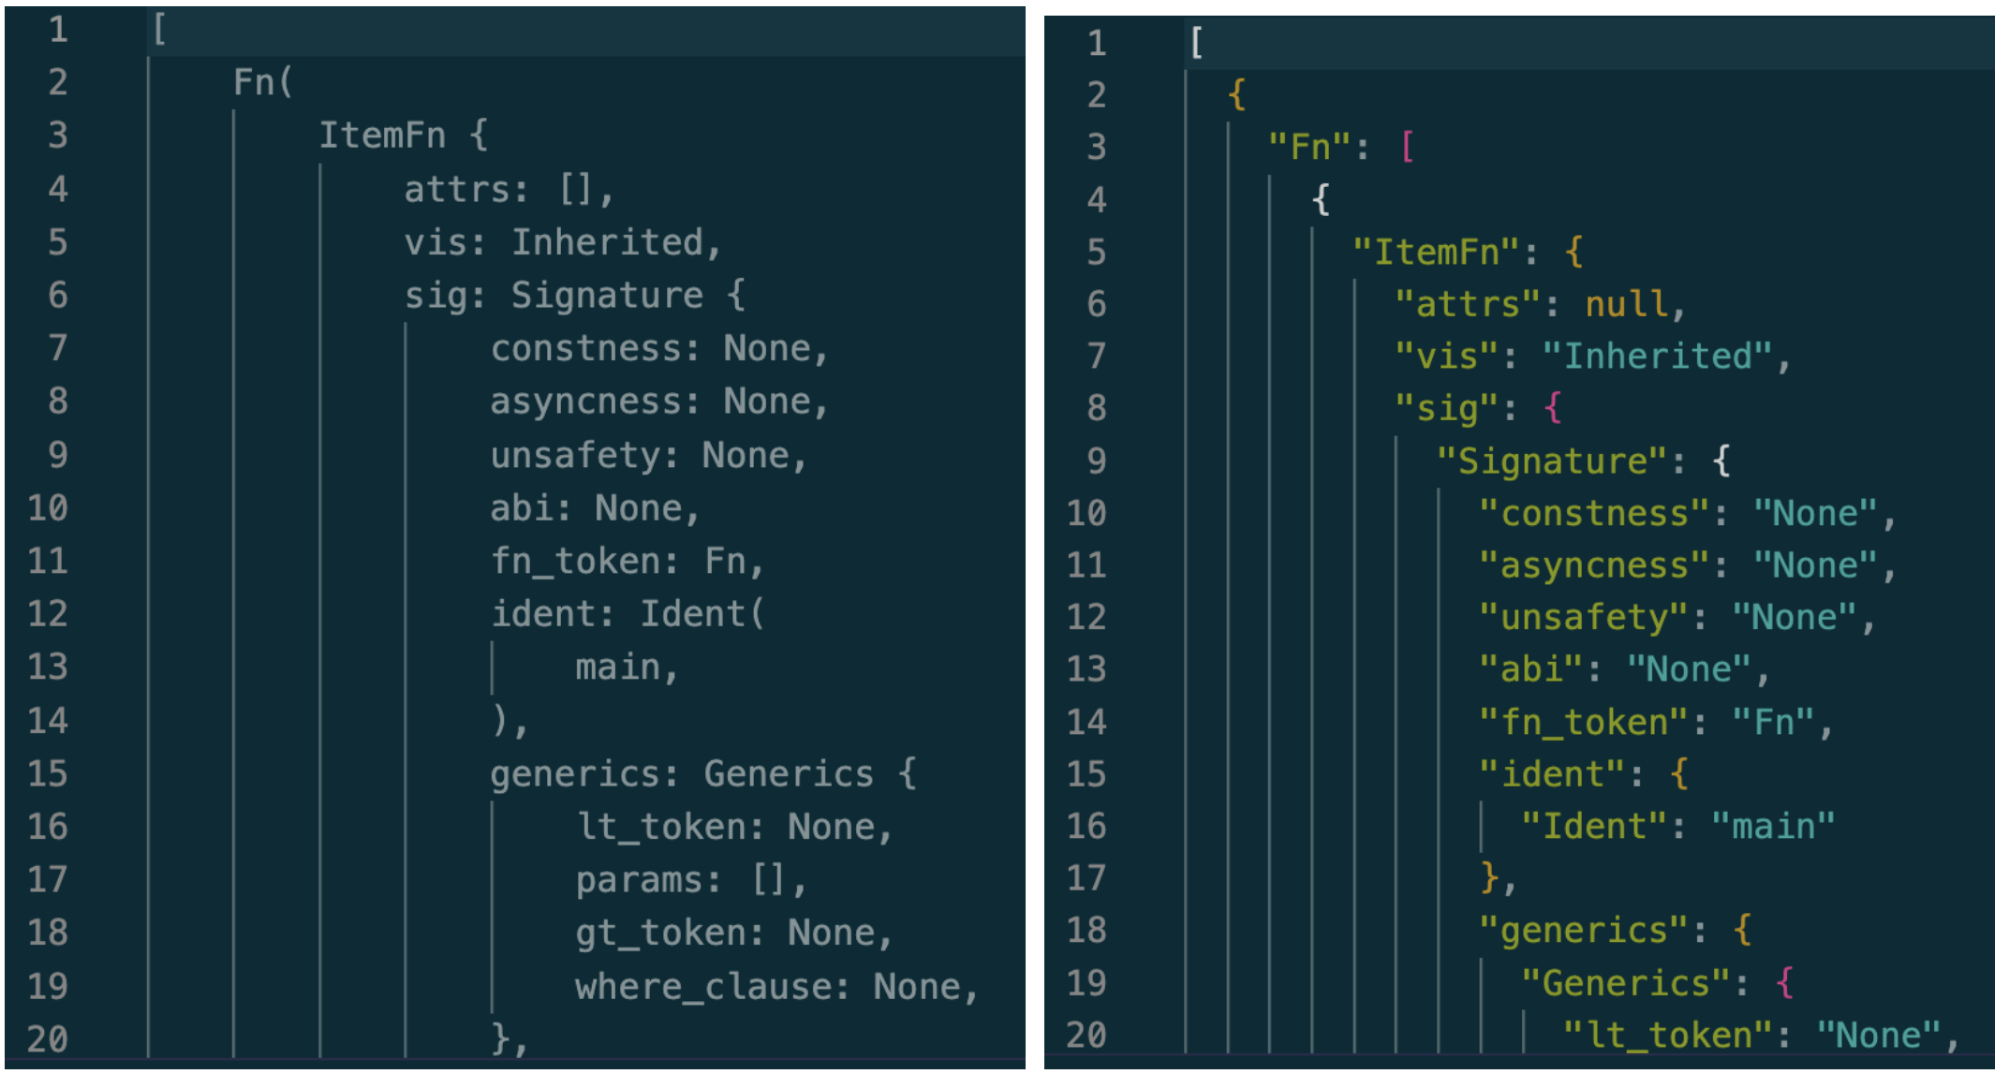
\includegraphics[width=1\textwidth]{astpics}
    \caption{Syn tree in Rust Debugging format (left) and Python dictionary format (right)}
\end{figure}

\subsubsection{\label{rev:2:path}Inconsistency between number of paths and the number of changed arguments}

\textit{\textbf{R2:} Second, I cannot understand Figure 1. What do the three paths represent? If they represent the changed parameters, why are there three paths, but there are only two parameters changed? If they represent parameters, how can they represent changes from the last version?}

\vspace*{1em} \noindent \textbf{Response:} This is a really good question. We added a few more sentences to make sure this doesn't confuse the readers. To clarify: the tree depicted in Figure 1 is not the actual AST; rather, it represents the ASTDiff (now written on the label on top left). In our approach, we consider two versions of the code: the buggy code and the fixed code. Consequently, we have two ASTs. The ASTDiff, shown in Figure 1, represents the difference between these two ASTs in Python dictionary format. The number of paths in the ASTDiff does not directly correspond to the number of changed elements in the source code. Instead, it is determined by the structural differences between the two ASTs of the code versions. The paths in the ASTDiff capture the changes in the code structure between the two versions, allowing us to analyze and extract relevant information for further processing. We have also added more text to Section 2.1.2 explaining this.

\vspace*{1em} \noindent \textit{\textbf{R2:} Third, I don't understand the following sentence on page 7: "we record the number of occurrences of items within the paths at each scope." Overall, the implementation can be benefited from a carefully described example.}

\vspace*{1em} \noindent \textbf{Response:} We revised the whole paragraph (now on page 8) and made the running example in Section 2 more explicit, as also requested by Reviewer 1. We meant that we record the number of occurrences of elements of \verb+NT+ $\cup$ \verb+BCE+ within each distinct root level scope. Root level scopes can be structs, functions, impl blocks, …. Note that Figure 2 does not explicitly show the single root level scope for this example, which is ItemFn. Other diffs could contribute items in different root level scopes. \\

\subsubsection{\label{rev:2:minor}Minor issues}

\textit{\textbf{R2:} 1. The introduction is organized in a very strange way. The authors should introduce Rust first, and then discuss studying common bug/fix patterns is important for Rust. However, the current writing does not mention Rust until the second page.}

\vspace*{1em} \noindent \textbf{Response:} Thanks. Moved Rust introduction to the beginning. \\ \\

\vspace*{1em} \noindent \textit{\textbf{R2:} 2. Line 15 on page 7: "We found it crucial to record" $\rightarrow$ it is crucial.}

\vspace*{1em} \noindent \textbf{Response:} fixed \\ \\

\vspace*{1em} \noindent \textit{\textbf{R2:} 3. The authors picked 50 datapoints for each cluster. Are there any particular reasons for choosing 50? There are very few clusters with more than 50 datapoints. A more reasonable method is to inspect all datapoints.}

\vspace*{1em} \noindent \textbf{Response:} Our analysis revealed many clusters (39 in total) with more than 50 datapoints. More specifically, one cluster has 618 datapoints, four clusters more than 300 datapoints, and 15 clusters more than 100 datapoints. With our number of datapoints, manual inspection would be overwhelmingly time-consuming.

We believe that the choice of 50 datapoints per cluster successfully balances ensuring that the selected datapoints truly represent the same change and making manual inspection feasible. Our sample size allows us to get meaningful insights into the characteristics of each cluster. \\ \\

\vspace*{1em} \noindent \textit{\textbf{R2:} 4. Line 6 on page 14: "A human analyzer (paper author) compares the actual change in the code and compares it to the visual representation of the respective data point." $\rightarrow$ A human analyzer (paper author) inspects the actual change … and compares it with the visual representation …}

\vspace*{1em} \noindent \textbf{Response:} fixed \\ \\

\vspace*{1em} \noindent \textit{\textbf{R2:} 5. What are the collected samples in the third paragraph of page 14 used for?}

\vspace*{1em} \noindent \textbf{Response:} We proposed a method to embed key AST information in a fixed-sized vector using a semi-automatically derived weighting scheme. RQ1 asks how successful we've been in terms of giving more values to the important elements in our ASTs. For instance, if in a code patch, the only change is adding \verb+.clone()+, then we should expect the element \verb+clone+ to have the highest value. In RQ1, we sample 25 datapoints from General datapoints and 25 datapoints from BC-related datapoints (50 in total) to manually analyze whether the values in their code vector actually respect the important elements in the AST. Note that we selected 50 datapoints that minimize the sampling error, i.e. it is a low bias sampling. \\ \\

\vspace*{1em} \noindent \textit{\textbf{R2:} 6. I don't understand the sentence at line 25 of page 23. Particularly, what string formatting methods are gone through if using p instead of *p?}

\vspace*{1em} \noindent \textbf{Response:} fixed, added Clippy reference in the paper. 

This is a common Clippy warning. You can find information about it through this link: \url{https://rust-lang.github.io/rust-clippy/master/index.html#inefficient_to_string} \\

In the link the example is: \\

\noindent\verb+// Generic implementation for `T: Display` is used (slow)+ \\
\verb+["foo", "bar"].iter().map(|s| s.to_string());+\\

\noindent\verb+// OK, the specialized impl is used+\\
\verb+["foo", "bar"].iter().map(|&s| s.to_string());+\\

It is the same as:

\noindent\verb+// Generic implementation for `T: Display` is used (slow)+\\
\verb+["foo", "bar"].iter().map(|s| s.to_string());+\\

\noindent\verb+// OK, the specialized impl is used+\\
\verb+["foo", "bar"].iter().map(|s| (*s).to_string());+\\

In summary, when \verb+p+ is used and it's not clear for Clippy that \verb+p+ cannot be of type \verb+&&T+ where \verb+T+ implements the \verb+ToString+ trait, it suggests dereferencing \verb+p+. The reason is that \verb+p.to_string()+ will use the \verb+format!()+ macro under the hood. The \verb+format!()+ macro is less efficient than direct casting of \verb+&T+ to String (probably because it allocates extra memory first then populates it based on formatting annotations). \verb+(*p).to_string()+ will not use \verb+format!()+.



\small
\bibliographystyle{plain}
\bibliography{refs}

\end{document}
